\documentclass[12pt]{article} 
% Custom definitions
% To use this customization file, insert the line "% Custom definitions
% To use this customization file, insert the line "% Custom definitions
% To use this customization file, insert the line "\input{custom}" in the header of the tex file.

% Formatting

\tolerance=1000
\usepackage[margin=1in]{geometry}


% Packages

% \usepackage{amssymb,latexsym}
\usepackage{amssymb,amsfonts,amsmath,latexsym,amsthm}
\usepackage[usenames,dvipsnames]{color}
\usepackage[]{graphicx}
\usepackage[space]{grffile}
\usepackage{mathrsfs}   % fancy math font
% \usepackage[font=small,skip=0pt]{caption}
\usepackage[skip=0pt]{caption}
\usepackage{subcaption}
\usepackage{verbatim}
\usepackage{url}
\usepackage{bm}
\usepackage{dsfont}
\usepackage{extarrows}
\usepackage{multirow}
% \usepackage{wrapfig}
% \usepackage{epstopdf}
\usepackage{rotating}
\usepackage{tikz}
\usetikzlibrary{fit}					% fitting shapes to coordinates
%\usetikzlibrary{backgrounds}	% drawing the background after the foreground

\usepackage{fancyhdr}

\fancypagestyle{firststyle}{
   \fancyhf{}
   \renewcommand{\footrulewidth}{0.4pt}
   \fancyfoot[L]{\footnotesize This work is licensed under a \href{http://creativecommons.org/licenses/by-nc-nd/4.0/}{Creative Commons BY-NC-ND 4.0 International License}.\\ Jeffrey W. Miller (2015). \textit{Lecture Notes on Bayesian Statistics}. Duke University, Durham, NC.}
}


% \usepackage[dvipdfm,colorlinks,citecolor=blue,linkcolor=blue,urlcolor=blue]{hyperref}
\usepackage[colorlinks,citecolor=blue,linkcolor=blue,urlcolor=blue]{hyperref}
%\usepackage{hyperref}
\usepackage[authoryear,round]{natbib}


%  Theorems, etc.

\theoremstyle{plain}
\newtheorem{theorem}{Theorem}[section]
\newtheorem{corollary}[theorem]{Corollary}
\newtheorem{lemma}[theorem]{Lemma}
\newtheorem{proposition}[theorem]{Proposition}
\newtheorem{condition}[theorem]{Condition}
% \newtheorem{conditions}[theorem]{Conditions}

\theoremstyle{definition}
\newtheorem{definition}[theorem]{Definition}
% \newtheorem*{unnumbered-definition}{Definition}
\newtheorem{example}[theorem]{Example}
\theoremstyle{remark}
\newtheorem*{remark}{Remark}
\numberwithin{equation}{section}



% Document-specific shortcuts
\newcommand{\btheta}{{\bm\theta}}
\newcommand{\bbtheta}{{\pmb{\bm\theta}}}

\newcommand{\commentary}[1]{\ifx\showcommentary\undefined\else \emph{#1}\fi}

\newcommand{\term}[1]{\textit{\textbf{#1}}}

% Math shortcuts

% Probability distributions
\DeclareMathOperator*{\Exp}{Exp}
\DeclareMathOperator*{\TExp}{TExp}
\DeclareMathOperator*{\Bernoulli}{Bernoulli}
\DeclareMathOperator*{\Beta}{Beta}
\DeclareMathOperator*{\Ga}{Gamma}
\DeclareMathOperator*{\TGamma}{TGamma}
\DeclareMathOperator*{\Poisson}{Poisson}
\DeclareMathOperator*{\Binomial}{Binomial}
\DeclareMathOperator*{\NormalGamma}{NormalGamma}
\DeclareMathOperator*{\InvGamma}{InvGamma}
\DeclareMathOperator*{\Cauchy}{Cauchy}
\DeclareMathOperator*{\Uniform}{Uniform}
\DeclareMathOperator*{\Gumbel}{Gumbel}
\DeclareMathOperator*{\Pareto}{Pareto}
\DeclareMathOperator*{\Mono}{Mono}
\DeclareMathOperator*{\Geometric}{Geometric}
\DeclareMathOperator*{\Wishart}{Wishart}

% Math operators
\DeclareMathOperator*{\argmin}{arg\,min}
\DeclareMathOperator*{\argmax}{arg\,max}
\DeclareMathOperator*{\Cov}{Cov}
\DeclareMathOperator*{\diag}{diag}
\DeclareMathOperator*{\median}{median}
\DeclareMathOperator*{\Vol}{Vol}

% Math characters
\newcommand{\R}{\mathbb{R}}
\newcommand{\Z}{\mathbb{Z}}
\newcommand{\E}{\mathbb{E}}
\renewcommand{\Pr}{\mathbb{P}}
\newcommand{\I}{\mathds{1}}
\newcommand{\V}{\mathbb{V}}

\newcommand{\A}{\mathcal{A}}
\newcommand{\C}{\mathcal{C}}
\newcommand{\D}{\mathcal{D}}
\newcommand{\Hcal}{\mathcal{H}}
\newcommand{\M}{\mathcal{M}}
\newcommand{\N}{\mathcal{N}}
\newcommand{\X}{\mathcal{X}}
\newcommand{\Zcal}{\mathcal{Z}}
\renewcommand{\P}{\mathcal{P}}

\newcommand{\T}{\mathtt{T}}
\renewcommand{\emptyset}{\varnothing}


% Miscellaneous commands
\newcommand{\iid}{\stackrel{\mathrm{iid}}{\sim}}
\newcommand{\matrixsmall}[1]{\bigl(\begin{smallmatrix}#1\end{smallmatrix} \bigr)}

\newcommand{\items}[1]{\begin{itemize} #1 \end{itemize}}

\newcommand{\todo}[1]{\emph{\textcolor{red}{(#1)}}}

\newcommand{\branch}[4]{
\left\{
	\begin{array}{ll}
		#1  & \mbox{if } #2 \\
		#3 & \mbox{if } #4
	\end{array}
\right.
}

% approximately proportional to
\def\app#1#2{%
  \mathrel{%
    \setbox0=\hbox{$#1\sim$}%
    \setbox2=\hbox{%
      \rlap{\hbox{$#1\propto$}}%
      \lower1.3\ht0\box0%
    }%
    \raise0.25\ht2\box2%
  }%
}
\def\approxprop{\mathpalette\app\relax}

% \newcommand{\approptoinn}[2]{\mathrel{\vcenter{
  % \offinterlineskip\halign{\hfil$##$\cr
    % #1\propto\cr\noalign{\kern2pt}#1\sim\cr\noalign{\kern-2pt}}}}}

% \newcommand{\approxpropto}{\mathpalette\approptoinn\relax}





" in the header of the tex file.

% Formatting

\tolerance=1000
\usepackage[margin=1in]{geometry}


% Packages

% \usepackage{amssymb,latexsym}
\usepackage{amssymb,amsfonts,amsmath,latexsym,amsthm}
\usepackage[usenames,dvipsnames]{color}
\usepackage[]{graphicx}
\usepackage[space]{grffile}
\usepackage{mathrsfs}   % fancy math font
% \usepackage[font=small,skip=0pt]{caption}
\usepackage[skip=0pt]{caption}
\usepackage{subcaption}
\usepackage{verbatim}
\usepackage{url}
\usepackage{bm}
\usepackage{dsfont}
\usepackage{extarrows}
\usepackage{multirow}
% \usepackage{wrapfig}
% \usepackage{epstopdf}
\usepackage{rotating}
\usepackage{tikz}
\usetikzlibrary{fit}					% fitting shapes to coordinates
%\usetikzlibrary{backgrounds}	% drawing the background after the foreground

\usepackage{fancyhdr}

\fancypagestyle{firststyle}{
   \fancyhf{}
   \renewcommand{\footrulewidth}{0.4pt}
   \fancyfoot[L]{\footnotesize This work is licensed under a \href{http://creativecommons.org/licenses/by-nc-nd/4.0/}{Creative Commons BY-NC-ND 4.0 International License}.\\ Jeffrey W. Miller (2015). \textit{Lecture Notes on Bayesian Statistics}. Duke University, Durham, NC.}
}


% \usepackage[dvipdfm,colorlinks,citecolor=blue,linkcolor=blue,urlcolor=blue]{hyperref}
\usepackage[colorlinks,citecolor=blue,linkcolor=blue,urlcolor=blue]{hyperref}
%\usepackage{hyperref}
\usepackage[authoryear,round]{natbib}


%  Theorems, etc.

\theoremstyle{plain}
\newtheorem{theorem}{Theorem}[section]
\newtheorem{corollary}[theorem]{Corollary}
\newtheorem{lemma}[theorem]{Lemma}
\newtheorem{proposition}[theorem]{Proposition}
\newtheorem{condition}[theorem]{Condition}
% \newtheorem{conditions}[theorem]{Conditions}

\theoremstyle{definition}
\newtheorem{definition}[theorem]{Definition}
% \newtheorem*{unnumbered-definition}{Definition}
\newtheorem{example}[theorem]{Example}
\theoremstyle{remark}
\newtheorem*{remark}{Remark}
\numberwithin{equation}{section}



% Document-specific shortcuts
\newcommand{\btheta}{{\bm\theta}}
\newcommand{\bbtheta}{{\pmb{\bm\theta}}}

\newcommand{\commentary}[1]{\ifx\showcommentary\undefined\else \emph{#1}\fi}

\newcommand{\term}[1]{\textit{\textbf{#1}}}

% Math shortcuts

% Probability distributions
\DeclareMathOperator*{\Exp}{Exp}
\DeclareMathOperator*{\TExp}{TExp}
\DeclareMathOperator*{\Bernoulli}{Bernoulli}
\DeclareMathOperator*{\Beta}{Beta}
\DeclareMathOperator*{\Ga}{Gamma}
\DeclareMathOperator*{\TGamma}{TGamma}
\DeclareMathOperator*{\Poisson}{Poisson}
\DeclareMathOperator*{\Binomial}{Binomial}
\DeclareMathOperator*{\NormalGamma}{NormalGamma}
\DeclareMathOperator*{\InvGamma}{InvGamma}
\DeclareMathOperator*{\Cauchy}{Cauchy}
\DeclareMathOperator*{\Uniform}{Uniform}
\DeclareMathOperator*{\Gumbel}{Gumbel}
\DeclareMathOperator*{\Pareto}{Pareto}
\DeclareMathOperator*{\Mono}{Mono}
\DeclareMathOperator*{\Geometric}{Geometric}
\DeclareMathOperator*{\Wishart}{Wishart}

% Math operators
\DeclareMathOperator*{\argmin}{arg\,min}
\DeclareMathOperator*{\argmax}{arg\,max}
\DeclareMathOperator*{\Cov}{Cov}
\DeclareMathOperator*{\diag}{diag}
\DeclareMathOperator*{\median}{median}
\DeclareMathOperator*{\Vol}{Vol}

% Math characters
\newcommand{\R}{\mathbb{R}}
\newcommand{\Z}{\mathbb{Z}}
\newcommand{\E}{\mathbb{E}}
\renewcommand{\Pr}{\mathbb{P}}
\newcommand{\I}{\mathds{1}}
\newcommand{\V}{\mathbb{V}}

\newcommand{\A}{\mathcal{A}}
\newcommand{\C}{\mathcal{C}}
\newcommand{\D}{\mathcal{D}}
\newcommand{\Hcal}{\mathcal{H}}
\newcommand{\M}{\mathcal{M}}
\newcommand{\N}{\mathcal{N}}
\newcommand{\X}{\mathcal{X}}
\newcommand{\Zcal}{\mathcal{Z}}
\renewcommand{\P}{\mathcal{P}}

\newcommand{\T}{\mathtt{T}}
\renewcommand{\emptyset}{\varnothing}


% Miscellaneous commands
\newcommand{\iid}{\stackrel{\mathrm{iid}}{\sim}}
\newcommand{\matrixsmall}[1]{\bigl(\begin{smallmatrix}#1\end{smallmatrix} \bigr)}

\newcommand{\items}[1]{\begin{itemize} #1 \end{itemize}}

\newcommand{\todo}[1]{\emph{\textcolor{red}{(#1)}}}

\newcommand{\branch}[4]{
\left\{
	\begin{array}{ll}
		#1  & \mbox{if } #2 \\
		#3 & \mbox{if } #4
	\end{array}
\right.
}

% approximately proportional to
\def\app#1#2{%
  \mathrel{%
    \setbox0=\hbox{$#1\sim$}%
    \setbox2=\hbox{%
      \rlap{\hbox{$#1\propto$}}%
      \lower1.3\ht0\box0%
    }%
    \raise0.25\ht2\box2%
  }%
}
\def\approxprop{\mathpalette\app\relax}

% \newcommand{\approptoinn}[2]{\mathrel{\vcenter{
  % \offinterlineskip\halign{\hfil$##$\cr
    % #1\propto\cr\noalign{\kern2pt}#1\sim\cr\noalign{\kern-2pt}}}}}

% \newcommand{\approxpropto}{\mathpalette\approptoinn\relax}





" in the header of the tex file.

% Formatting

\tolerance=1000
\usepackage[margin=1in]{geometry}


% Packages

% \usepackage{amssymb,latexsym}
\usepackage{amssymb,amsfonts,amsmath,latexsym,amsthm}
\usepackage[usenames,dvipsnames]{color}
\usepackage[]{graphicx}
\usepackage[space]{grffile}
\usepackage{mathrsfs}   % fancy math font
% \usepackage[font=small,skip=0pt]{caption}
\usepackage[skip=0pt]{caption}
\usepackage{subcaption}
\usepackage{verbatim}
\usepackage{url}
\usepackage{bm}
\usepackage{dsfont}
\usepackage{extarrows}
\usepackage{multirow}
% \usepackage{wrapfig}
% \usepackage{epstopdf}
\usepackage{rotating}
\usepackage{tikz}
\usetikzlibrary{fit}					% fitting shapes to coordinates
%\usetikzlibrary{backgrounds}	% drawing the background after the foreground

\usepackage{fancyhdr}

\fancypagestyle{firststyle}{
   \fancyhf{}
   \renewcommand{\footrulewidth}{0.4pt}
   \fancyfoot[L]{\footnotesize This work is licensed under a \href{http://creativecommons.org/licenses/by-nc-nd/4.0/}{Creative Commons BY-NC-ND 4.0 International License}.\\ Jeffrey W. Miller (2015). \textit{Lecture Notes on Bayesian Statistics}. Duke University, Durham, NC.}
}


% \usepackage[dvipdfm,colorlinks,citecolor=blue,linkcolor=blue,urlcolor=blue]{hyperref}
\usepackage[colorlinks,citecolor=blue,linkcolor=blue,urlcolor=blue]{hyperref}
%\usepackage{hyperref}
\usepackage[authoryear,round]{natbib}


%  Theorems, etc.

\theoremstyle{plain}
\newtheorem{theorem}{Theorem}[section]
\newtheorem{corollary}[theorem]{Corollary}
\newtheorem{lemma}[theorem]{Lemma}
\newtheorem{proposition}[theorem]{Proposition}
\newtheorem{condition}[theorem]{Condition}
% \newtheorem{conditions}[theorem]{Conditions}

\theoremstyle{definition}
\newtheorem{definition}[theorem]{Definition}
% \newtheorem*{unnumbered-definition}{Definition}
\newtheorem{example}[theorem]{Example}
\theoremstyle{remark}
\newtheorem*{remark}{Remark}
\numberwithin{equation}{section}



% Document-specific shortcuts
\newcommand{\btheta}{{\bm\theta}}
\newcommand{\bbtheta}{{\pmb{\bm\theta}}}

\newcommand{\commentary}[1]{\ifx\showcommentary\undefined\else \emph{#1}\fi}

\newcommand{\term}[1]{\textit{\textbf{#1}}}

% Math shortcuts

% Probability distributions
\DeclareMathOperator*{\Exp}{Exp}
\DeclareMathOperator*{\TExp}{TExp}
\DeclareMathOperator*{\Bernoulli}{Bernoulli}
\DeclareMathOperator*{\Beta}{Beta}
\DeclareMathOperator*{\Ga}{Gamma}
\DeclareMathOperator*{\TGamma}{TGamma}
\DeclareMathOperator*{\Poisson}{Poisson}
\DeclareMathOperator*{\Binomial}{Binomial}
\DeclareMathOperator*{\NormalGamma}{NormalGamma}
\DeclareMathOperator*{\InvGamma}{InvGamma}
\DeclareMathOperator*{\Cauchy}{Cauchy}
\DeclareMathOperator*{\Uniform}{Uniform}
\DeclareMathOperator*{\Gumbel}{Gumbel}
\DeclareMathOperator*{\Pareto}{Pareto}
\DeclareMathOperator*{\Mono}{Mono}
\DeclareMathOperator*{\Geometric}{Geometric}
\DeclareMathOperator*{\Wishart}{Wishart}

% Math operators
\DeclareMathOperator*{\argmin}{arg\,min}
\DeclareMathOperator*{\argmax}{arg\,max}
\DeclareMathOperator*{\Cov}{Cov}
\DeclareMathOperator*{\diag}{diag}
\DeclareMathOperator*{\median}{median}
\DeclareMathOperator*{\Vol}{Vol}

% Math characters
\newcommand{\R}{\mathbb{R}}
\newcommand{\Z}{\mathbb{Z}}
\newcommand{\E}{\mathbb{E}}
\renewcommand{\Pr}{\mathbb{P}}
\newcommand{\I}{\mathds{1}}
\newcommand{\V}{\mathbb{V}}

\newcommand{\A}{\mathcal{A}}
\newcommand{\C}{\mathcal{C}}
\newcommand{\D}{\mathcal{D}}
\newcommand{\Hcal}{\mathcal{H}}
\newcommand{\M}{\mathcal{M}}
\newcommand{\N}{\mathcal{N}}
\newcommand{\X}{\mathcal{X}}
\newcommand{\Zcal}{\mathcal{Z}}
\renewcommand{\P}{\mathcal{P}}

\newcommand{\T}{\mathtt{T}}
\renewcommand{\emptyset}{\varnothing}


% Miscellaneous commands
\newcommand{\iid}{\stackrel{\mathrm{iid}}{\sim}}
\newcommand{\matrixsmall}[1]{\bigl(\begin{smallmatrix}#1\end{smallmatrix} \bigr)}

\newcommand{\items}[1]{\begin{itemize} #1 \end{itemize}}

\newcommand{\todo}[1]{\emph{\textcolor{red}{(#1)}}}

\newcommand{\branch}[4]{
\left\{
	\begin{array}{ll}
		#1  & \mbox{if } #2 \\
		#3 & \mbox{if } #4
	\end{array}
\right.
}

% approximately proportional to
\def\app#1#2{%
  \mathrel{%
    \setbox0=\hbox{$#1\sim$}%
    \setbox2=\hbox{%
      \rlap{\hbox{$#1\propto$}}%
      \lower1.3\ht0\box0%
    }%
    \raise0.25\ht2\box2%
  }%
}
\def\approxprop{\mathpalette\app\relax}

% \newcommand{\approptoinn}[2]{\mathrel{\vcenter{
  % \offinterlineskip\halign{\hfil$##$\cr
    % #1\propto\cr\noalign{\kern2pt}#1\sim\cr\noalign{\kern-2pt}}}}}

% \newcommand{\approxpropto}{\mathpalette\approptoinn\relax}






% Latex Listings language definition/style for Julia
% Source: https://gist.github.com/chi-feng/6589066
%         Github User "chi-feng"
% License: UNKNOWN
% Date accessed: 12/30/2014

% \usepackage{inconsolata} % very nice fixed-width font included with texlive-full
\usepackage{zi4} % EDIT: inconsolata is now accessed through zi4
\usepackage[usenames,dvipsnames]{color} % more flexible names for syntax highlighting colors
\usepackage{listings}
 
\lstset{
basicstyle=\ttfamily, 
columns=fullflexible, % make sure to use fixed-width font, CM typewriter is NOT fixed width
numbers=left, 
numberstyle=\small\ttfamily\color{Gray},
stepnumber=1,              
numbersep=10pt, 
numberfirstline=true, 
numberblanklines=true, 
tabsize=4,
lineskip=-1.5pt,
extendedchars=true,
breaklines=true,        
keywordstyle=\color{Blue}\bfseries,
identifierstyle=, % using emph or index keywords
commentstyle=\sffamily\color{OliveGreen},
stringstyle=\color{Maroon},
showstringspaces=false,
showtabs=false,
upquote=false,
texcl=true % interpet comments as LaTeX
}
 
\lstdefinelanguage{julia}
{
  keywordsprefix=\@,
  morekeywords={
    exit,whos,edit,load,is,isa,isequal,typeof,tuple,ntuple,uid,hash,finalizer,convert,promote,
    subtype,typemin,typemax,realmin,realmax,sizeof,eps,promote_type,method_exists,applicable,
    invoke,dlopen,dlsym,system,error,throw,assert,new,Inf,Nan,pi,im,begin,while,for,in,return,
    break,continue,macro,quote,let,if,elseif,else,try,catch,end,bitstype,ccall,do,using,module,
    import,export,importall,baremodule,immutable,local,global,const,Bool,Int,Int8,Int16,Int32,
    Int64,Uint,Uint8,Uint16,Uint32,Uint64,Float32,Float64,Complex64,Complex128,Any,Nothing,None,
    function,type,typealias,abstract
  },
  sensitive=true,
  morecomment=[l]{\#},
  morestring=[b]',
  morestring=[b]" 
}

\graphicspath{{figures/}}
\def\showcommentary{1}


\title{Chapter 6: Solutions to Exercises}
\author{}
\date{}


\begin{document}
\maketitle
\thispagestyle{firststyle}


\subsection*{Exercise 1}

\subsubsection*{Part (a)}
\begin{align*}
    p(x|y) &\underset{x}{\propto} \I(|x-y|<c)\I(0<x<1)\\
        &= \I(y-c<x<y+c)\I(0<x<1)\\
        &= \I(\max\{0,y-c\}<x<\min\{1,y+c\})\\
        &\underset{x}{\propto} \Uniform\big(x\mid \max\{0,y-c\},\,\min\{1,y+c\}\big).
\end{align*}
By symmetry,
$$ p(y|x) = \Uniform\big(y\mid (\max\{0,x-c\},\,\min\{1,x+c\})\big). $$
Hence, the Gibbs sampler (in the $(x,y)$ parametrization) is to initialize $x,y$ and then alternately sample:
\begin{align*}
     X|y\,\sim\,\Uniform(\max\{0,y-c\},\,\min\{1,y+c\}),\\
     Y|x\,\sim\,\Uniform(\max\{0,x-c\},\,\min\{1,x+c\}).
\end{align*}

\subsubsection*{Part (b)}
See code in Appendix.

\subsubsection*{Part (c)}
See Figure \ref{figure:box}.

\begin{figure}
    \centering
    \begin{subfigure}[t]{1\textwidth}
        \centering
            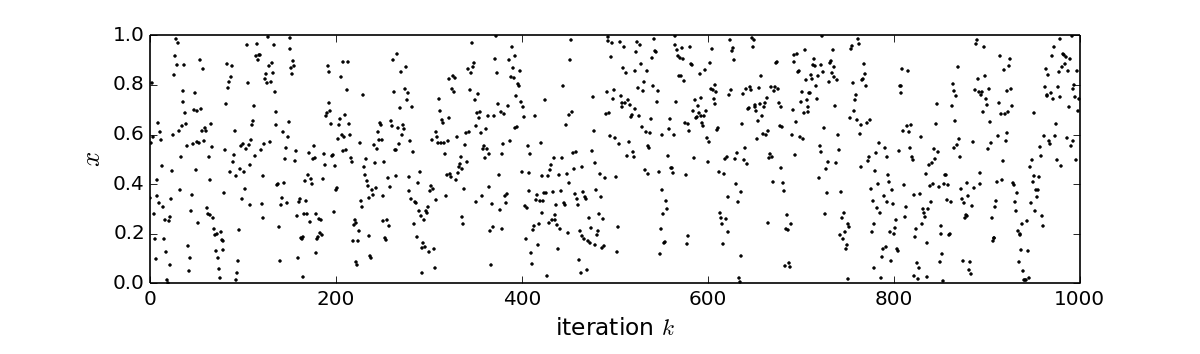
\includegraphics[trim=0 0.4cm 0 0, clip, width=0.9\textwidth]{code/box-x_trace-c=0.25.png}
            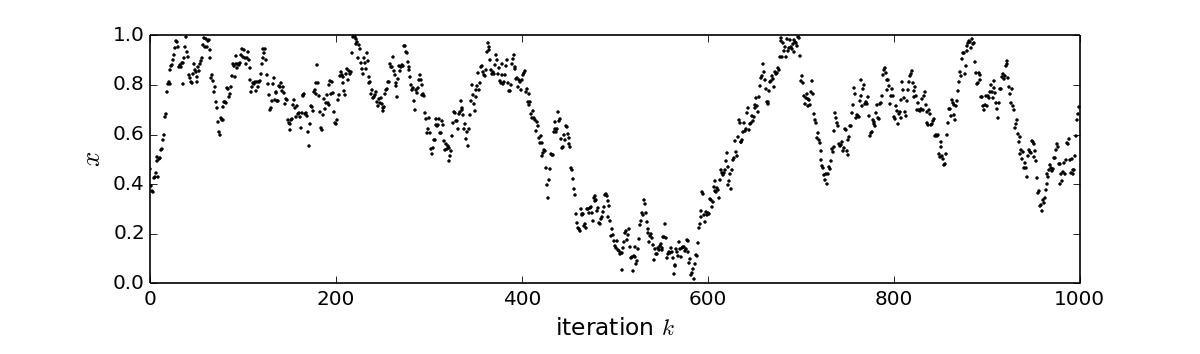
\includegraphics[trim=0 0.4cm 0 0, clip, width=0.9\textwidth]{code/box-x_trace-c=0.05.png}
            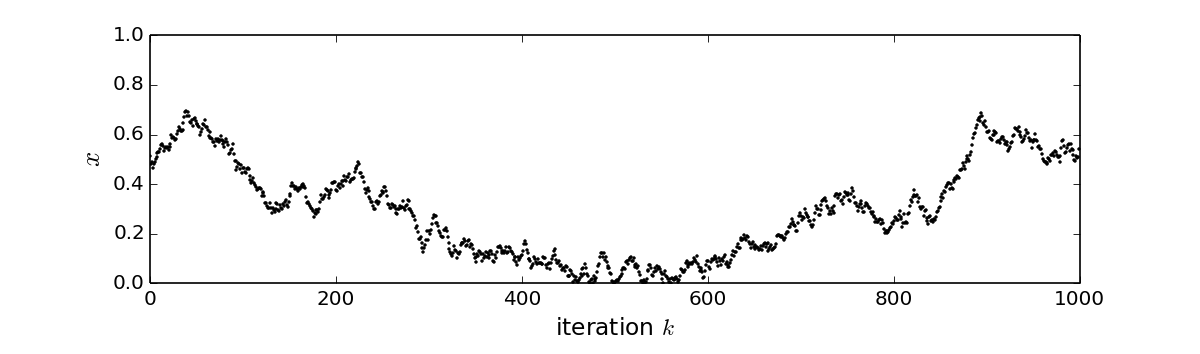
\includegraphics[trim=0 0.4cm 0 0, clip, width=0.9\textwidth]{code/box-x_trace-c=0.02.png}
        % Original work by Jeffrey W. Miller
        \caption{Traceplots of $x$ for $c = 0.25$, $c = 0.05$, and $c = 0.02$.}
    \end{subfigure}
    \begin{subfigure}[t]{1\textwidth}
        \centering
            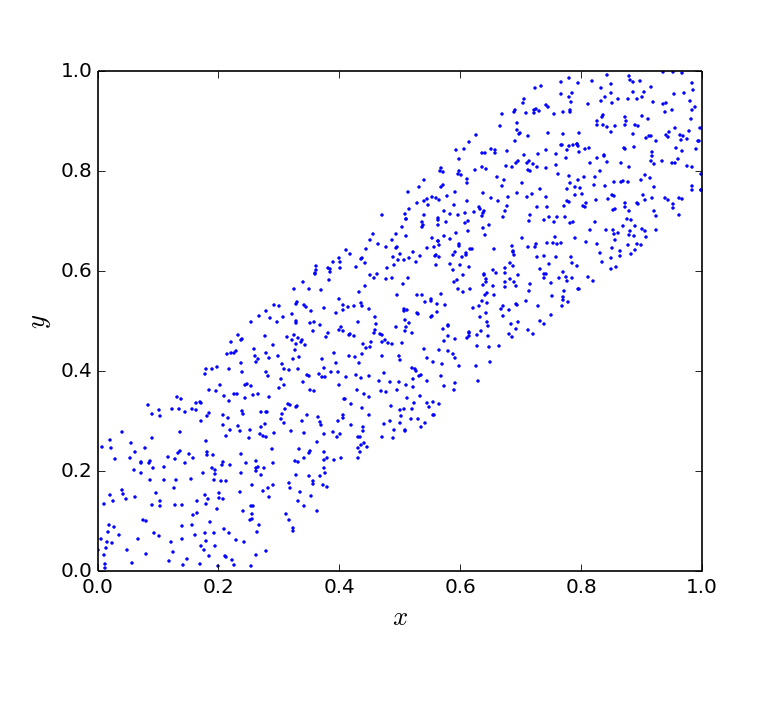
\includegraphics[trim=0.8cm 0.4cm 0.8cm 0, clip, width=0.325\textwidth]{code/box-scatter-c=0.25.png}
            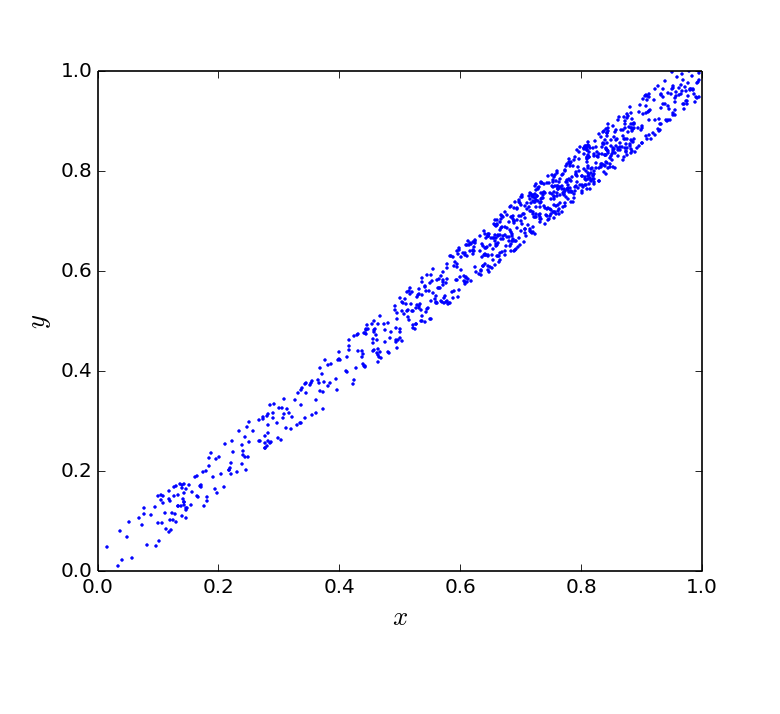
\includegraphics[trim=0.8cm 0.4cm 0.8cm 0, clip, width=0.325\textwidth]{code/box-scatter-c=0.05.png}
            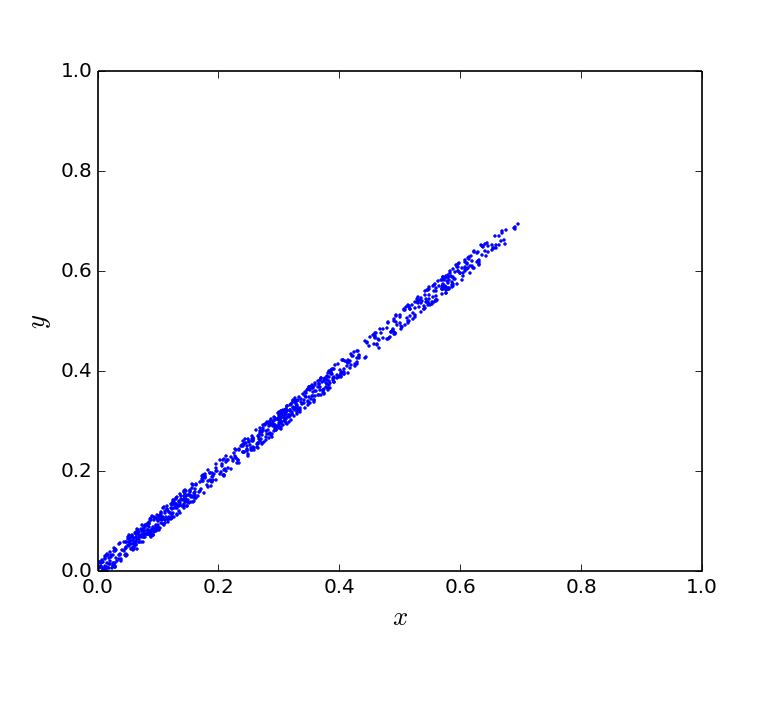
\includegraphics[trim=0.8cm 0.4cm 0.8cm 0, clip, width=0.325\textwidth]{code/box-scatter-c=0.02.png}
        % Original work by Jeffrey W. Miller
        \caption{Scatterplots of $(x,y)$ samples for $c = 0.25$, $c = 0.05$, and $c = 0.02$.}
    \end{subfigure}
    \vspace{.5em}
    \caption{Results for Exercise 1.}
    \label{figure:box}
\end{figure}

\subsubsection*{Part (d)}
The issue is that when $c$ is small, the range of each variable is highly restricted, given the other variable. As a result, the sampler has
to make many ``zig--zag'' moves in order to travel long distances (see Figure \ref{figure:box-short}). 
This causes the correlation between successive samples to be high when $c$ is small, as we can see in the traceplots of $x$---the traceplot
indicates that it takes a long time to see significant changes in the samples. This makes the performance of the sampler worse---it
takes many more samples to achieve the same level of accuracy when making approximations based on these samples.

\begin{figure}
  \begin{center}
      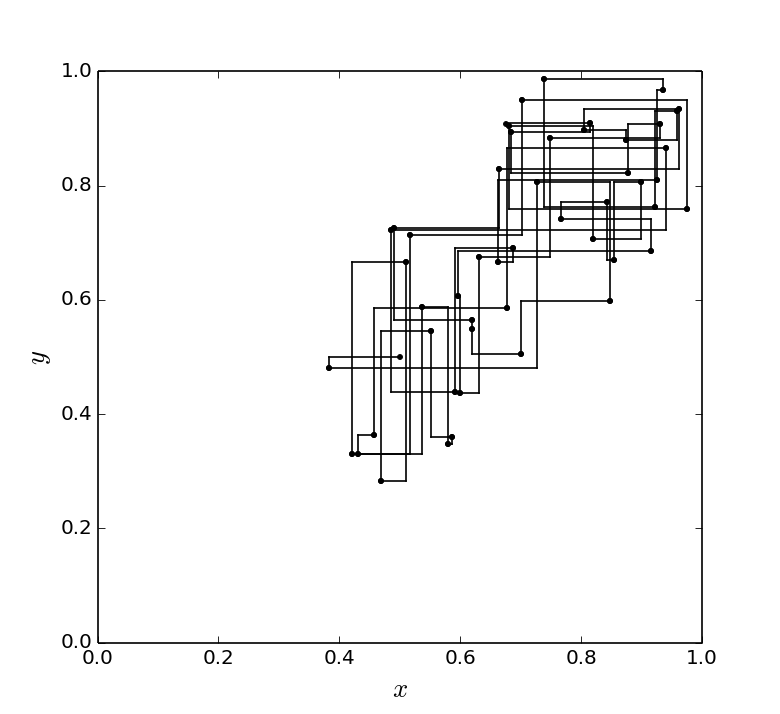
\includegraphics[width=0.48\textwidth]{code/box-walk-c=0.25.png}
      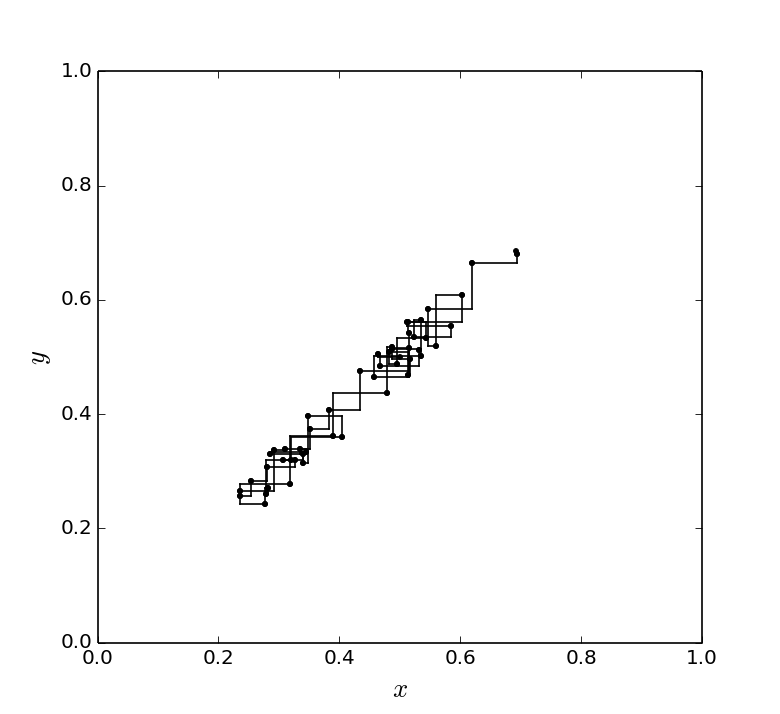
\includegraphics[width=0.48\textwidth]{code/box-walk-c=0.05.png}
      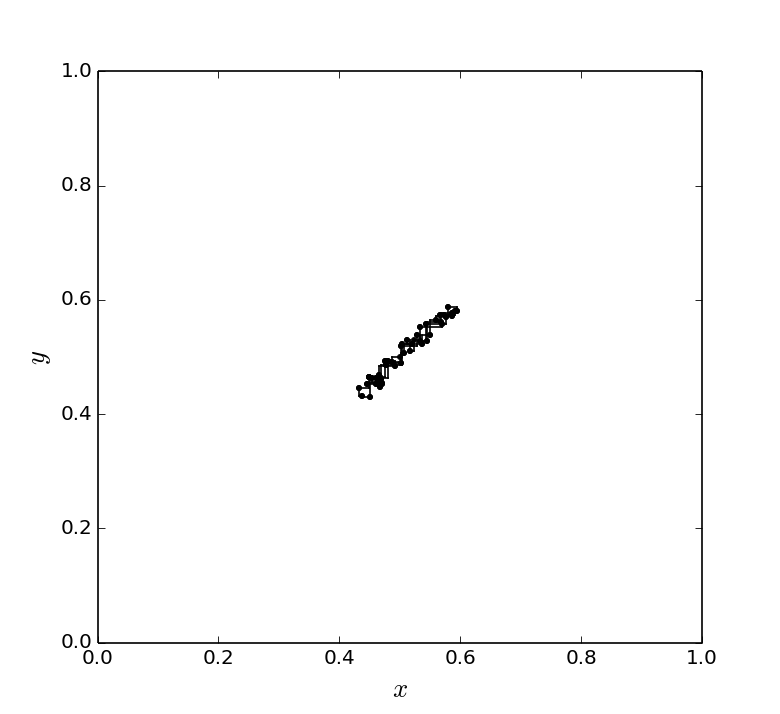
\includegraphics[width=0.48\textwidth]{code/box-walk-c=0.02.png}
    % Source: Original work by J. W. Miller.
  \end{center}
    \caption{Path of the Gibbs sampler for first few $(x,y)$ samples, for $c = 0.25$, $c = 0.05$, and $c = 0.02$.}
  \label{figure:box-short}
\end{figure}


\subsection*{Exercise 2}

\subsubsection*{Part (a)}
\begin{align*}
    p(u|v) &\underset{u}{\propto} \I(|v|<u<1-|v|)
    \underset{u}{\propto} \Uniform\big(u\,\big\vert\, |v|,1-|v|\big)\\
    p(v|u) &\underset{v}{\propto} \I(|v|<c/2)\I(|v|<u<1-|v|) \\
    &=\left\{
        \begin{array}{ll}
            -u<v<u & \text{if } u\leq c/2 \\
            -c/2<v<c/2 & \text{if } c/2<u\leq 1-c/2 \\
            u-1<v<1-u & \text{if } 1-c/2<u
        \end{array}
    \right.\\
    &\propto\left\{
        \begin{array}{ll}
            \Uniform(v\mid -u,u) & \text{if } u\leq c/2 \\
            \Uniform(v\mid -c/2,c/2) & \text{if } c/2<u\leq 1-c/2 \\
            \Uniform(v\mid u-1,1-u) & \text{if } 1-c/2<u
        \end{array}
    \right.
\end{align*}

\subsubsection*{Part (b)}
See code in Appendix.

\subsubsection*{Part (c)}
See Figure \ref{figure:box-transformed}.
The reason why this works so much better is that $u$ can move long distances, given $v$ --- the strong coupling that was present between $x$
and $y$ is not exhibited by $u$ and $v$. This significantly reduces the correlation between samples, and will result in far better
approximation accuracy for the same number of samples.

\begin{figure}
    \centering
    \begin{subfigure}[t]{1\textwidth}
        \centering
            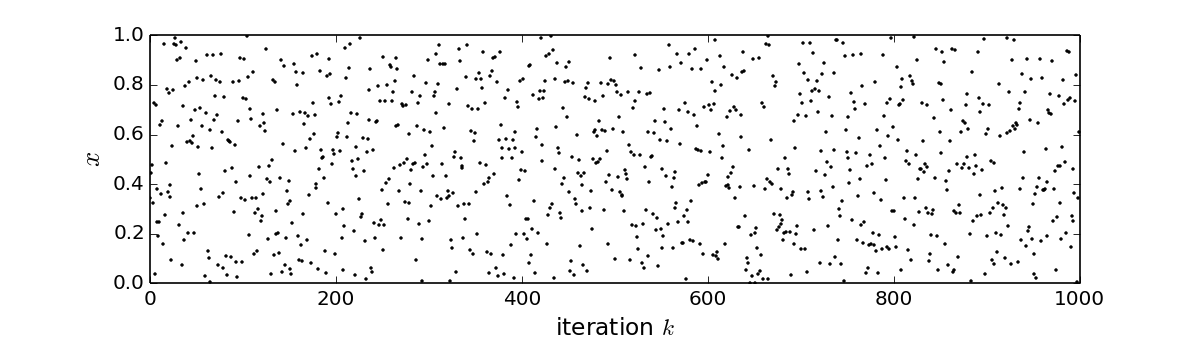
\includegraphics[trim=0 0.4cm 0 0, clip, width=0.9\textwidth]{code/box-x_trace-c=0.25-transformed.png}
            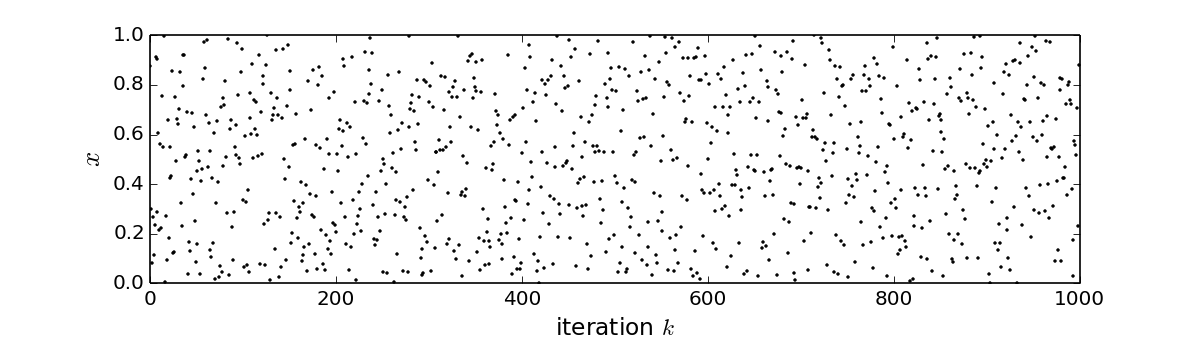
\includegraphics[trim=0 0.4cm 0 0, clip, width=0.9\textwidth]{code/box-x_trace-c=0.05-transformed.png}
            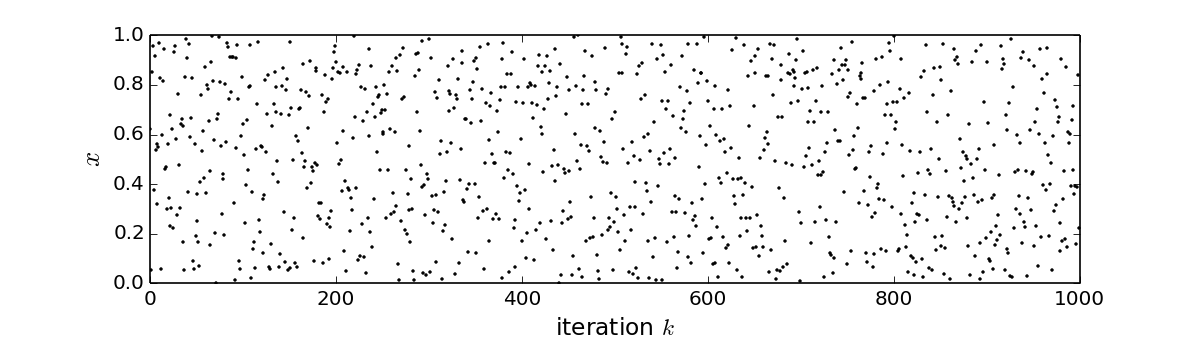
\includegraphics[trim=0 0.4cm 0 0, clip, width=0.9\textwidth]{code/box-x_trace-c=0.02-transformed.png}
        % Original work by Jeffrey W. Miller
        \caption{Traceplots of $x$ for $c = 0.25$, $c = 0.05$, and $c = 0.02$.}
    \end{subfigure}
    \begin{subfigure}[t]{1\textwidth}
        \centering
            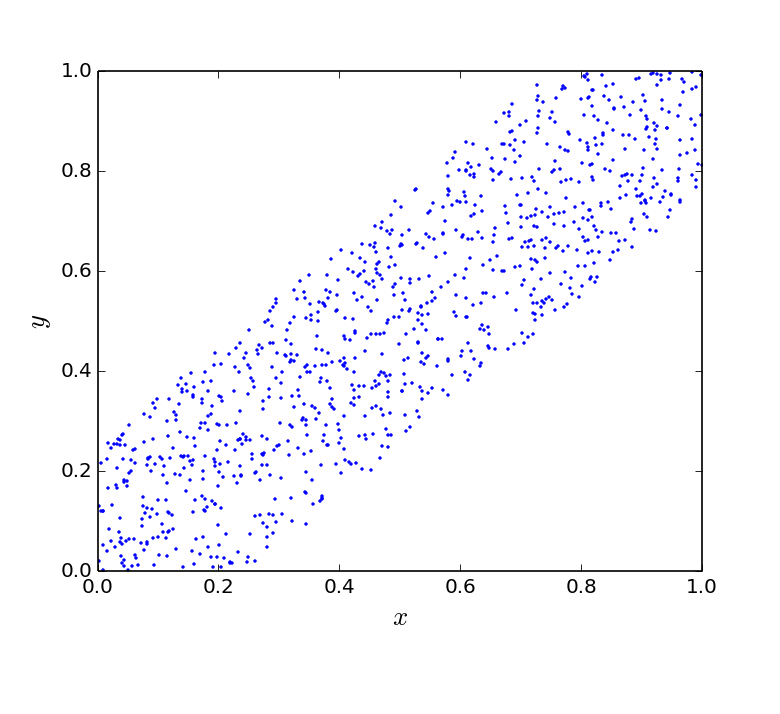
\includegraphics[trim=0.8cm 0.4cm 0.8cm 0, clip, width=0.325\textwidth]{code/box-scatter-c=0.25-transformed.png}
            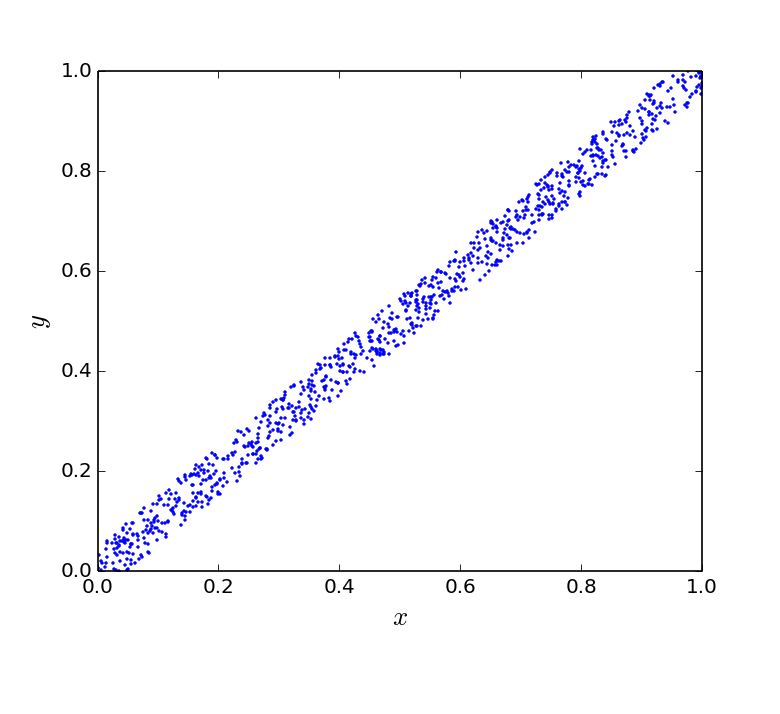
\includegraphics[trim=0.8cm 0.4cm 0.8cm 0, clip, width=0.325\textwidth]{code/box-scatter-c=0.05-transformed.png}
            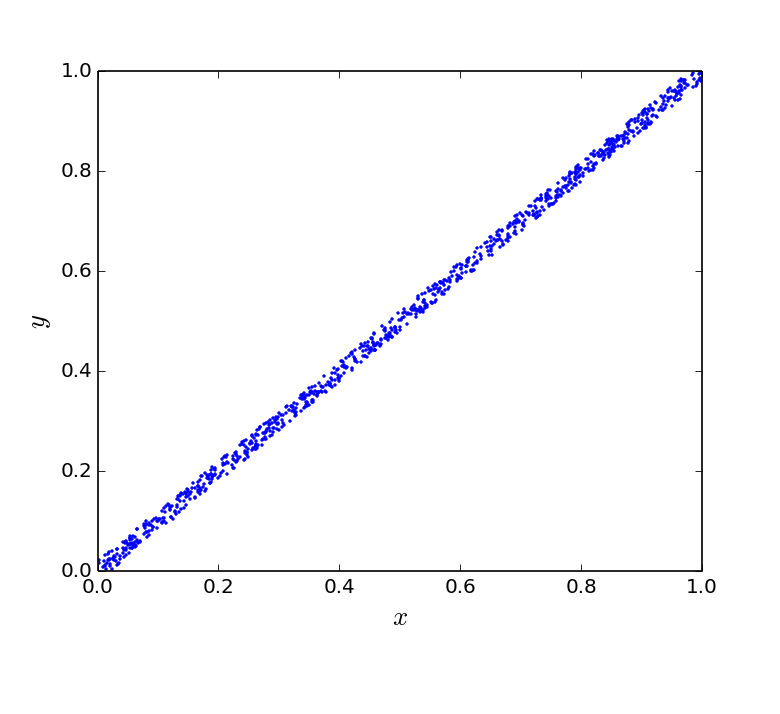
\includegraphics[trim=0.8cm 0.4cm 0.8cm 0, clip, width=0.325\textwidth]{code/box-scatter-c=0.02-transformed.png}
        % Original work by Jeffrey W. Miller
        \caption{Scatterplots of $(x,y)$ samples for $c = 0.25$, $c = 0.05$, and $c = 0.02$.}
    \end{subfigure}
    \vspace{.5em}
    \caption{Results for Exercise 2, using transformed Gibbs sampler.}
    \label{figure:box-transformed}
\end{figure}




\appendix
\section{Source code in Julia language}

\subsection*{Exercises 1 and 2}
\lstinputlisting[language=julia,numbers=none,commentstyle=\tt\color{OliveGreen},firstline=1]{code/box-solution.jl}



\end{document}






